\subsection{Gegensprechanlage}

Mit dem Einbau von synchroner Sprachübertragung wird das Praxisrufsystem um die Funktion Gegensprechanlage erweitert.
Die gewählte Technologie WebRTC erlaubt es Peer-to-Peer Sprachverbindungen zwischen Clients aufzubauen.
Dieses Kapitel beschreibt wie das Praxisrufsystem erweitert wird, um eine konfigurierbare Gegensprechanlage mit WebRTC zu integrieren.

\subsubsection{Konfiguration}

Die Gegensprechanlage wird in den nativen Mobile Client integriert.
Praxismitarbeitende können über Buttons Sprachverbindungen zu anderen Clients aufbauen.
Welche Buttons und damit welche Sprachverbindungen zur Verfügung stehen, wird durch Praxisadministrierende über das Admin UI konfiguriert.
Damit dies möglich ist, sind Änderungen an der Domäne Configuration des Cloudservice sowie am Admin UI notwendig.

Die Konfiguration von Mobile Clients wird in der Domäne Configuration abgebildet.
Zentral sind dabei die beiden Entities Client und ClientConfiguration.
Ein Client repräsentiert ein physisches Endgerät.
Eine ClientConfiguration definiert die Konfiguration eines Gerätes.

Praxisruf bietet bereits heute die Möglichkeit Buttons zu konfigurieren, über welche Benachrichtigungen versendet werden können.
Diese Buttons werden mit der Entität NotificationType konfiguriert, welche wiederum einer ClientConfiguration zugeordnet werden können.
Diese ClientConfiguration wird bei der Anmeldung auf dem Mobile Client geladen und verwendet, um die nötigen Buttons darzustellen.
Für die Konfiguration von Sprachverbindungen wird die Entität CallType erstellt.
Ein CallType beinhaltet den Text, welcher auf dem zugehörigen Button auf Clientseite angezeigt wird und eine Liste von Clients, welche als Ziel der Sprachverbindung verwendet werden.
Abbildung 7.12 zeigt einen Ausschnitt aus dem Entity Relationship Diagramm der Configuration Domäne.
Dabei sind die Teile, die für die Konfiguration von Sprachverbindungen ergänzt werden, grün markiert.

\begin{figure}[h]
    \centering
    \begin{minipage}[b]{0.7\textwidth}
        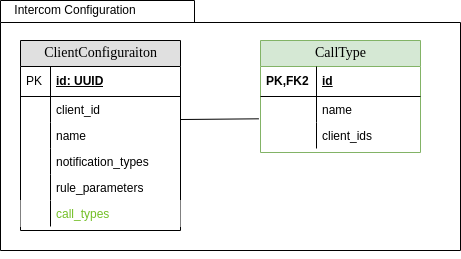
\includegraphics[width=\textwidth]{/home/joshua/FHNW/dev/IP6/IP6_Bachelorarbeit_Bericht_Cloudbasiertes_Praxisrufsystem/src/graphics/diagramms/erd_intercom_v02.drawio}
        \caption{ERD Ausschnitt - Konfiguration Gegensprechanlage}
    \end{minipage}
\end{figure}

Das Admin UI wird mit Ansichten erweitert, um CallTypes zu erstellen, anzeigen, bearbeiten und löschen.
Gleichzeitig wird der Cloudservice um Rest Endpunkte für das Lesen, Erstellen, Aktualisieren und Löschen von CallTypes erweitert.
Die Ansichten für ClientConfigurations im Admin UI werden so erweitert, dass CallTypes darauf angezeigt, hinzugefügt und entfernt werden können.
Die bestehenden Endpunkte für ClientConfiguration werden entsprechend erweitert.

\clearpage

\subsubsection{Signaling Instanz}

Mit WebRTC werden Peer-To-Peer Verbindungen aufgebaut~\cite{webrtc}.
Damit diese Verbindungen aufgebaut werden können, müssen die beteiligten Geräte Signalmeldungen austauschen können.
Dazu ist eine Instanz notwendig, welche Signale zwischen den Endgeräten vermitteln kann.
Diese Signaling Instanz wird als Teil des Cloudservice implementiert.

%Prinzipiell ist es möglich, den Signalaustausch in dieses Modul zu integrieren.
%Dieser Ansatz hat aber zwei grosse Probleme.
%Erstens ist die Grösse von Medlungen, welche über den gewählten Messaging Service (Firebase Cloud Messaging) ausgetauscht werden können beschränkt.
%Meldungen zum Aufbau von WebRTC Verbindungen können diese Grösse überschreiten.\footnote{cite}
%Zweitens geschieht das Versenden von Benachrichtigungen über einen asynchronen Mechanismus.
%Die Signale für Sprachverbindungen sollen aber synchron ausgetauscht werden.
%Es soll unmittelbar beim Versuch des Verbindungsaufbau klar sein, ob die Verbindung etabliert werden kann oder nicht.
%Diese Id entspricht der technischen Identifikation des entsprechenden Mobile Clients und muss, wenn sich der Mobile Client für eine Verbindung registriert mitgesendet werden.

Der Cloudservice wird um ein neues Modul ''Signaling'' erweitert.
Dieses soll den Austausch von Signalen zwischen Clients ermöglichen.
Gleich wie das Modul für Sprachsynthese wird es unabhängig von den anderen Domänenmodulen im Cloudservice implementiert.
Das Modul Signaling muss dabei zwei Aufgaben übernehmen.
Erstens muss es Mobile Clients die Möglichkeit bieten, sich für Sprachverbindungen zu registrieren.
Zu diesem Zweck müssen Mobile Clients eine Verbindung mit der Signaling Instanz herstellen und trennen können.
Zweitens muss es Signalmeldungen empfangen und an die relevanten Empfänger zustellen können.
Kann eine Signalmeldung nicht zugestellt werden, muss es den betroffenen Empfänger über das verpasste Signal informieren.

Für diese Funktionen wird das Interface ClientConnector definiert.
Dieses definiert die Methoden afterConnectionEstablished und afterConnectionClosed.
Die beiden Methoden werden aufgerufen, wenn eine Verbindung geöffnet bzw.\ geschlossen wurde.
Die Implementierung dieses Interfaces ist dafür verantwortlich verfügbare Verbindungen zu verwalten.
Weiter definiert das Interface die Methode handleSignal.
Diese muss verwendet werden, um ein Signal entgegenzunehmen und an relevante Empfänger weiterzuleiten.

\begin{figure}[h]
    \centering
    \begin{minipage}[b]{1\textwidth}
        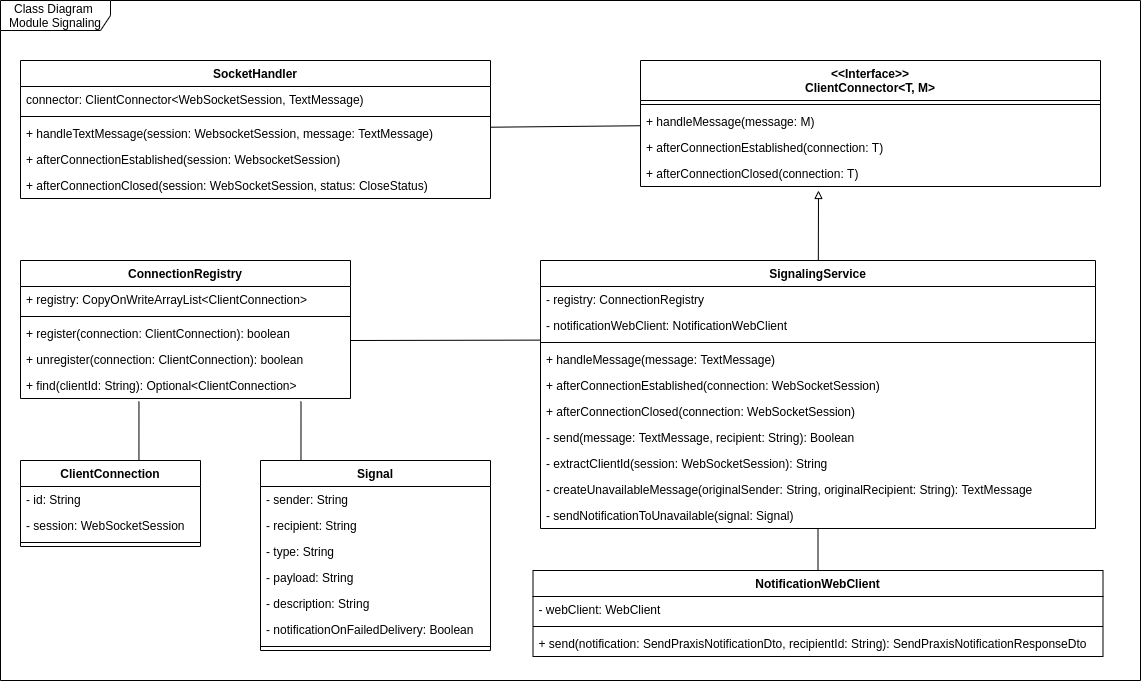
\includegraphics[width=\textwidth]{/home/joshua/FHNW/dev/IP6/IP6_Bachelorarbeit_Bericht_Cloudbasiertes_Praxisrufsystem/src/graphics/diagramms/Class_Intercom_Full_V01}
        \caption{Klassendiagramm SpeechSynthesisController}
    \end{minipage}
\end{figure}

Die Klasse SignalingService implementiert das ClientConnector Interface.
Der SignalingService führt eine Liste an verfügbaren Verbindungen.
Dabei wird jede Verbindung durch eine eindeutige Id gekennzeichnet.
Für die Verwaltung von Verbindungen wird die Komponente ConnectionRegistry implementiert.
Diese muss Verbindungen anhand einer Id registrieren und wieder entfernen können.
Weiter müssen Verbindungen anhand ihrer Id gefunden werden können.
Für das Zustellen von Signalen über bekannte Verbindungen wird die Methode handleSignal implementiert.
Jedes Signal muss die Identifikation seines Empfängers beinhalten.
Beim Empfang eines Signals wird kontrolliert, ob die ConnectionRegistry eine Verbindung für die Identifikation des Empfängers enthält.
Ist dies der Fall, wird das Signal über diese Verbindung an den Empfänger übermittelt.
Wenn dies nicht der Fall ist oder wenn das Senden des Signals fehlschlägt, ist der Empfänger nicht erreichbar.
Nicht erreichbare Empfänger werden mit Benachrichtigungen über verpasste Signale informiert.
Dazu wird eine Benachrichtigung über die API des Moduls Notification versendet.

Die Schnittestelle der Signaling Instanz im Cloudservice wird mit Websockets umgesetzt.
Dazu wird die Bibliothek Spring-Boot-Starter-Websocket verwendet.
Es wird ein WebsocketHandler implementiert, welcher unter dem Pfad ''$<$serverUrl$>$/signaling'' erreichbar ist.
Etablierte Verbindungen müssen eindeutig einem Client zugeordnet werden können.
Diese Identifikation wird als Query Parameter bei Verbindungsaufbau mitgegeben.
Der WebsocketHandler definiert Methoden die beim Öffnen und Schliessen von Verbindungen aufgerufen werden.
Diese delegieren das Verwalten der Verbindungen an den SignalingService.
Empfangene Meldungen werden an den SignalingService übergeben und wie oben beschrieben verarbeitet.

\subsubsection{Signaling Security}

Der Zugriff auf den Signaling Service darf nur für Berechtigte möglich sein.
Um dies sicherzustellen, wird der Verbindungsaufbau nur erlaubt, wenn die Anfrage dazu authentisiert ist.
Für die Authentisierung wird derselbe Mechanismus wie für Http Anfragen in den anderen Cloudservice Domänen verwendet werden.
Über die SecurityConfig des Cloudservices wird die Authentifizierung aller Http Requests überprüft.
Mit dieser Prüfung wird sichergestellt, dass ein gültiges JWT Token im Authentication Header der Anfrage vorhanden ist.
Wenn kein gültiges Token vorhanden ist, wird eine entsprechende Fehlermeldung zurückgegeben.
Der Aufbau der Websocketverbindung wird abgebrochen.

Mit der Klasse HttpSessionHandshakeInterceptor kann vor dem Aufbau einer Websocketverbindung geprüft werden, dass der Http Request für den Verbindungsaufbau authentifiziert wurde.
Mit der Verarbeitung des Http Requests durch die SecurityConfig des Cloudservices wurden die Rollen, welche dem Aufrufer zugeteilt ausgelesen.
Im HttpSessionHandshakeInterceptor können diese Informationen ausgewertet und geprüft werden, dass ein Benutzer für den Austausch von Signalmeldungen authorisiert ist.
Ist er dies nicht, wird der Aufbau der Websocketverbindung wird abgebrochen und eine Fehlermeldung zurückgegeben.
Das Praxisrufsystem kennt die zwei Rollen ''ADMIN'' und ''USER''.
Beide Rollen sind berechtigt, dass Rufsystem über den Mobile Client zu verwenden und dürfen damit Signalmeldungen austauschen.

Für den Aufbau von Websockets wird das ausschliesslich das Protokoll Secure WebSockets (WSS) verwendet.
Der Austausch von Signalmeldungen ist damit verschlüsselt.

\clearpage

\subsubsection{Signalmeldungen}

Dieses Kapitel beschreibt die Signalmeldungen, welche für Sprachverbindungen verwendet werden.
Abbildung 7.14 zeigt, wie Signalmeldungen im Mobile Client modeliert werden.

\begin{figure}[h]
    \centering
    \begin{minipage}[b]{0.33\textwidth}
        \fbox{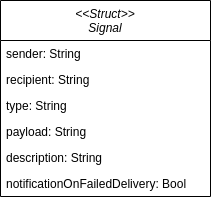
\includegraphics[width=\textwidth]{graphics/diagramms/Class_Signal_V01}}
        \caption{Signal }
    \end{minipage}
\end{figure}

Alle Signalmeldungen beinhalten Identifikation von Sender und Empfänger.
Diese werden vom Signalingserver verwendet, um die Signale korrekt weiterzuleiten.
Type, Payload und Description werden im Mobile Client verwendet, um das Signal korrekt zu verarbeiten und Verbindungen aufzubauen.
Das Flag notificationOnFailedDelivery wird im Cloudservice ausgewertet.
Wenn ein Signal nicht zugestellt werden kann und dieses Flag TRUE ist, wird der Empfänger mit einer asynchrone Benachrichtigung darüber informiert.
Dazu wird das bestehende Notification Modul des Cloudservices verwendet.
Für die Verwaltung von Sprachverbindungen werden die folgenden sechs Typen von Signalmeldungen definiert.
\\ \\
\begin{tabbing}
    Left \= Middle \= Right \= Right \kill
    Offer
    \> \> \> Ein Offer wird vom Initiator der Sprachverbindung an die Empfänger gesendet. Es
    \\\> \> \> beinhaltet die Informationen des Initiators. \\ \\

    Answer
    \> \> \> Eine Answer wird vom Empfänger eines Offers an den Initiator der Sprachverbindung
    \\\> \> \> gesendet. Es beinhaltet SDP Informationen des Empfängers. \\ \\

    Ice Candidate
    \> \> \> Ice Candidate Signal Beinhaltet Informatinoen eines ICE Candidates, die für den Ver-
    \\ \> \> \> bindungsaufbau verwendet werden. Nach Verarbeitung von Offer und Answer
    \\ \> \> \> tauschen Initiator und Empfänger solange Ice Candidate Signale aus, bis sie sich auf
    \\ \> \> \> einen Kandidaten geeinigt haben.\\ \\

    End
    \> \> \> Wird von Empfänger oder Initiator versendet, nachdem die Verbindung durch tippen des
    \\ \> \> \> Auflegen-Button in der Applikation beendet wurde. Empfang dieses Signal führt dazu,
    \\ \> \> \> dass offene Sprachverbindungen zum Sender dieses Signals beendet werden.\\ \\

    Unavailable
    \> \> \> Wenn der Signalingserver ein Signal nicht zustellen kann, wird das Ziel über eine Benach-
    \\ \> \> \> richtigung informiert. Zudem wird ein Unavailable Signal zurück an den Sender gesendet.
    \\ \> \> \> Es wird angezeigt, dass der gewünschte gesprächspartner nicht verfügbar ist. \\ \\

    Decline
    \> \> \> Wird ein Signal empfangen während die Gegensprechanlage in den lokalen Einstellungen
    \\ \> \> \> deaktiviert ist, sendet der Mobile Client ein Decline Signal zurück. Es wird angezeigt,
    \\ \> \> \>  dass der gewünschte gesprächspartner nicht verfügbar ist.
\end{tabbing}

\subsubsection{Anmeldung und Registrierung}

Der Ablauf von Anmeldung und Registrierung funktioniert mit dem neuen nativen Mobile Client grundsätzlich gleich wie zuvor.
Praxismitarbeitende öffnen die Applikation und geben ihr Benutzername und Passwort ein.
Der Mobile Client verwendet diese um sich über Basic Authentication beim Cloudservice anzumelden.
Als Antowrt auf die Anmeldung gibt der Cloudservice ein JWT Token zurück.
Dieses wird für die Authentifizierung aller weiteren Anfragen an den Cloudservice verwendet.
Nachdem die Anmeldung erfolgt ist, wird eine Liste der verfügbaren Konfigurationen geladen.
Der Benutzer wählt die gewünschte Konfiguration aus und bestätigt.

\begin{figure}[h]
    \centering
    \begin{minipage}[b]{0.9\textwidth}
        \fbox{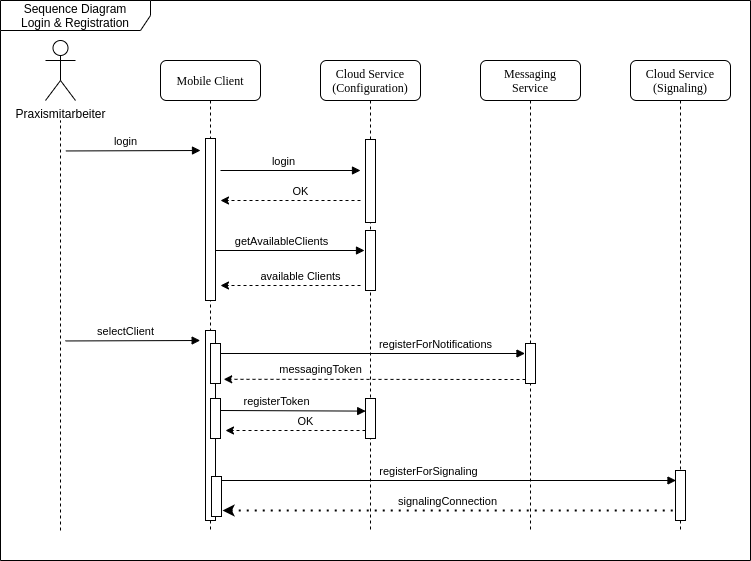
\includegraphics[width=\textwidth]{/home/joshua/FHNW/dev/IP6/IP6_Bachelorarbeit_Bericht_Cloudbasiertes_Praxisrufsystem/src/graphics/diagramms/Sequence_Registration}}
        \caption{Sequenzdiagramm - Anmeldung und Registrierung im Mobile Client}
    \end{minipage}
\end{figure}

Danach wird diese Konfiguration geladen und die Hauptansicht angezeigt.
Die geladene Konfiguration beinhaltet alle Informationen die nötig sind um Buttons für Benachrichtigungen und Sprachverbindungen anzuzeigen.
Im Hintergrund muss sich der Mobile Client nun für Benachrichtigungen und Sprachverbindungen registrieren.
Für Benachrichtigungen registriert er sich zuerst bei Firebase Cloud Messaging.
Er erhält ein Token, welches den Client beim Messaging Service identifiziert.
Dieses Token sendet der Mobile Client zusammen mit der gewählten Konfiguration an den Cloudservice.
Dieser persistiert die Registrierung und kann sie verwenden, um Benachrichtigungen an diesen Client zuzustellen.
Für Sprachverbindungen muss zudem eine Verbindung zum Signaling Modul des Cloudservices aufgebaut werden.
Dazu wird wie in Kapitel 7.4.6 beschrieben eine Websocketverbindung geöffnet.

\clearpage

\subsubsection{Verbindungsaufbau}

Praxismitarbeitende können Sprachverbindungen zu anderen Clients aufbauen indem sie auf den entsprechenden Button in der Praxisruf App tippen.
Zum Zeitpunkt an dem der Button getippt wird, weiss der Mobile Client noch nicht, zu welchen Clients diese Verbindung aufgebaut werden soll.
Als erstes muss deshalb beim Cloudservice angefragt werden, welche Clients mit dem betätigten Button angesprochen werden sollen.
Der Cloudservice bietet dazu einen Endpoint an über den der vollständige CallType des verwendeten Buttons hinterlegt sind geladen werden können.
Nachdem diese Informationen geladen sind, können Sprachverbindungen zu allen relevanten Clients aufgebaut werden.
Dazu müssen Offer, Answer und Ice Candidate Signale ausgetauscht werden.
Der auslösende Client initialisiert die Peer to Peer Verbindung auf seiner Seite und sendet für jeden Gesprächspartner ein Offer.
Der Cloudservice findet die Verbindung der relevanten Empfänger und leitet die Signale über die jeweilige Verbindung weiter.
Die Verbindung auf Empfängerseite wird nach Eingang des Offers initialisiert.
Danach wird eine Answer zurück an den Initiator gesendet, welche über den Signalingserver zugestellt wird,
Der Initiator empfängt die Antwort Signale und ergänzt die notwendigen Verbindungsinformationen.
Abbildung 7.15 visualisiert diesen Ablauf.

\begin{figure}[h]
    \centering
    \begin{minipage}[b]{0.9\textwidth}
        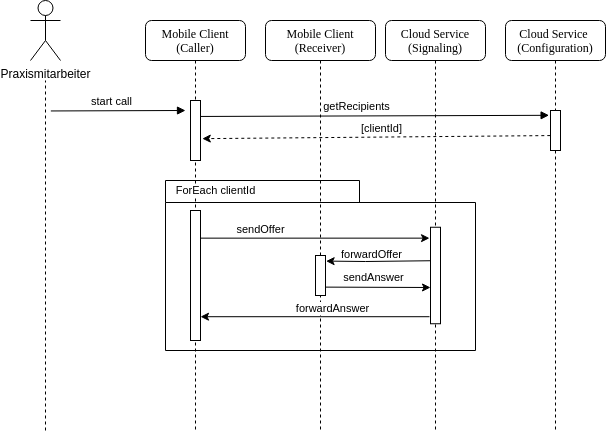
\includegraphics[width=\textwidth]{graphics/diagramms/Sequence_Intercom_Broking_V02}
        \caption{Ablauf Verbindungsaufbau Gegensprechanlage}
    \end{minipage}
\end{figure}

Nachdem die Offer und Answer Meldungen ausgetauscht sind, müssen Ice Candidate Meldungen ausgetauscht werden.
Dieser Austausch ist der um die Übersichtlichkeit zu wahren nicht in Abbildung 7.15 dargestellt.
Er verläuft nach demselben Prinzip wie der Austausch von Offer und Answer.
Sobald sich die Clients auf die Verbindungsinformationen geeinigt haben, besteht die Sprachverbindung.

\clearpage

\subsubsection{Anbindung Mobile Client an Singaling Instanz}

Für den Aufbau von Sprachverbindungen zwischen Mobile Clients müssen mehrere Signalmeldungen ausgetauscht werden.
Der Cloud Service wird im Rahmen dieses Projektes um eine Schnittstelle erweitert, welche dies ermöglicht.
Als Technologie für diese Schnittstelle werden Websockets verwendet.
Der Service PraxisrufApi wird dementsprechend erweitert, um Websocket Verbindungen zu ermöglichen.
Dies beinhaltet den Auf- und Abbau von Websocket Verbindungen, sowie das Senden und Empfangen von Meldungen über diese Verbindung.
Die Verbindung zur Signaling Instanz konstant offen gehalten und im Fehlerfall erneut aufgebaut werden können.

Der Austausch von Signalmeldungen ist der einzige Anwendungsfall in Praxisruf, der Websocketverbindungen benötigt.
Deshalb wird auf eine generische Integration von Verbindungen analog von Http Verbindungen verzichtet.
Es werden die Extension PraxisrufApi+Signaling und das Protokoll PraxisrufApiSignalingDelegate definiert, wie in Abbildung 7.17 dargestellt implementiert.

\begin{figure}[h]
    \centering
    \begin{minipage}[b]{0.9\textwidth}
        \fbox{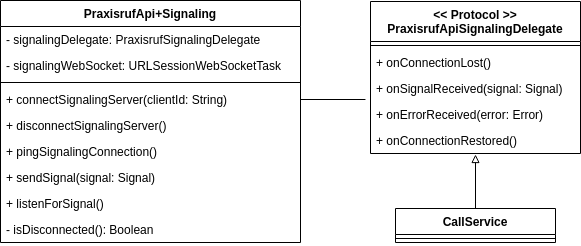
\includegraphics[width=\textwidth]{graphics/diagramms/Class_Mobile_Client_Signaling_Connection}}
        \caption{Klassendiagramm - Signaling Schnittstelle in Mobile Client}
    \end{minipage}
\end{figure}

Die Extension PraxisrufApi+Signaling ist für die Verbindung zu der Signaling Instanz verantwortlich.
Für die Integration dieser Extension in den Rest der Applikation wird das Protokoll PraxisrufApiSignalingDelegate definiert.

Die Verbindung zu der Signaling Instanz wird direkt nach der Anmeldung im Mobile Client aufgebaut.
Dazu wird die Methode connectSignalingServer verwendet.
Die Identifikation des Clients wird bei dieser Abfrage als Parameter mitgegeben.
So kann die Verbindung von der Signaling Instanz eindeutig einem Client zugeordnet werden.
Nachdem die Verbindung geöffnet ist, dürfen Signale empfangen und verarbeitet werden.
Dies wird durch die Methode listenForSignal initialisiert.
Darin wird der Websocketverbindung signalisiert, dass der Client bereit ist die nächste Meldung zu empfangen.
Sobald eine Meldung empfangen wird, wird diese über PraxisrufApiSignalingDelegate verarbeitet.

Für die Verarbeitung von Meldungen wird die entsprechende Methode des PraxisrufApiSignalingDelegate verwendet.
Wurde eine gültige Signalmeldung empfangen, wird diese über die Methode onSignalReceived verarbeitet.
Wurde hingegen eine ungültige Signalmeldung oder eine Fehlermeldung empfangen wird die Methode onErrorReceived aufgerufen.
Im Fehlerfall wird zudem überprüft ob die Verbindung noch offen verwendbar ist.
Sollte die Verbindung nicht mehr verwendbar sein, wird die Methode onConnectionLost des Delegates aufgerufen.

PraxisrufApi+Signaling definiert weiter Methoden um Signal- und Pingmeldungen zu versenden.
Pingmeldungen werden in Regelmässigen Abständen gesendet um sicherzustellen, dass die Verbindung zu der Signaling Instanz stabil ist.
Vor dem Senden einer Meldung wird geprüft, ob die Verbindung zur Signaling Instanz verwendbar ist.
Ist dies nicht der Fall, wird die Methode onConnectionLost des Delegates aufgerufen und anschliessend versucht die Meldung zu versenden.
Schlägt das Senden fehl, wird onErrorReceived auf dem Delegate aufgerufen.

Die Methoden des Protokolls CallClientDelegate werden durch die Klasse CallService implementiert.
Der CallService vermittelt Anfragen zwischen Signaling Instanz, Benutzeroberfläche und der Integration der Peer-To-Peer Verbindungen im Mobile Client.
Er ist dafür verantwortlich Signale an die Peer-To-Peer Verbindung weiterzuleiten, geschlossene Verbindungen wieder zu öffnen und Fehlermeldungen anzuzeigen.
Das Wiederöffnen der Verbindung im Fehlerfall wird über die PraxsirufApi+Signaling Extension gemacht.
Der entsprechende Aufruf wird aber im CallService implementiert.
Dadurch können allfällige Fehlermeldungen angezeigt und Benutzerinteraktionen ermöglicht werden.

\subsubsection{Sprachverbindungen im Mobile Client}

Der Mobile Client muss Signale verarbeiten und die Peer-To-Peer Sprachverbindungen über die WebRTC Bibliothek verwalten.
Für die Integration der WebRTC-Komponenten wird eine Klasse CallClient und ein Protokoll CallClientDelegate erstellt.
Diese sind für das Verwalten von Sprachverbindungen verantwortlich.
Abbildung 7.18 zeigt das Klassendiagramm beider Komponenten.

\begin{figure}[h]
    \centering
    \begin{minipage}[b]{0.6\textwidth}
        \fbox{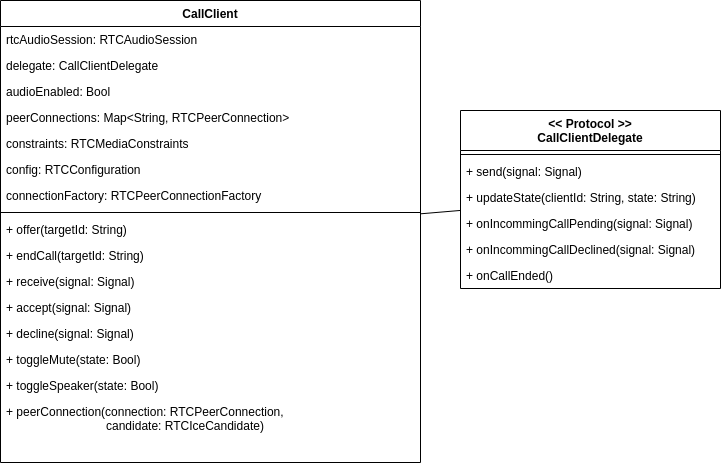
\includegraphics[width=\textwidth]{graphics/diagramms/Class_Mobile_Client_Signal_Processing}}
        \caption{Klassendiagramm - CallClient und CallClientDelegate}
    \end{minipage}
\end{figure}

Für den Aufbau von ausgehenden Verbindungen wird eine RTCPeerConnection im CallClient des Senders initialisiert.
Es werden die SDP Informationen für Beschreibung der Verbindung erstellt und mit einem Offer-Signal an den Empfänger gesendet.
Das Offer-Signal wird über die Signaling Instanz an den Empfänger zugestellt.
Der CallClient des Empfängers erstellt bei Empfang des Offer-Signals eine RTCPeerConnection anhand der darin enthaltenen SDP Informationen.
Anschliessend erstellt er ein Answer-Signal und sendet dieses zurück an den Verbindungspartner.
Das Answer-Signal wird vom Initiator der Verbindung verarbeitet, um die Verbindung zu bestätigen.
Signale werden im CallClient durch die Methode receive empfangen und über die Methode send des CallClientDelegates versendet.

Neben dem Austausch von Offer- und Answer-Signalen müssen Ice Candidate Signale ausgetauscht werden können.
Sobald ein Ice Candidate zur Verfügung steht, erstellt der CallClient ein entsprechendes Signal und sendet es an den Empfänger.
Damit dies möglich ist, muss der CallClient über verfügbare Ice Candidates informeirt werden.
Die WebRTC Bibliothek bietet dazu das Protokoll RTCPeerConnectionDelegate.
Dieses kann auf der RTCPeerConnection registriert werden und wird aufgerufen, sobald ein neuer Ice Candidate verfügbar ist.
Der CallClient implementiert dieses Protokoll und registriert sich auf allen RTCPeerConnections.

Sprachverbindungen müssen über die Benutzeroberfläche verwaltet werden können.
Der CallClient bietet deshalb Methoden an, um eine Verbindung zu starten und beenden.
Weiter bietet er die Möglichkeit Mikrofon und Lautsprecher für geöffnete Verbindungen stummzuschalten.
Bei eingehenden Verbindungen, dem Beenden von Anrufen und Veränderungen am Status einer Verbindung, muss die Benutzeroberfläche informiert werden.
Der CallClientDelegate definiert dazu Methoden über welche der CallClient diese Informationen weitergeben kann.

\subsubsection{Signalverarbeitung im Mobile Client}

Peer-To-Peer Sprachverbindungen werden über die Komponenten CalService, CallClient und PraxisrufApi+Signaling in den Mobile Client integriert.
Dieses Kapitel beschreibt den Kommunikationsablauf zwischen diesen Komponenten.

CallClient und PraxisrufApi+Signaling definieren je ein Delegate-Protokoll.
Diese Protokolle definieren die Funktionen, über welche die Komponenten Informationen weitergeben können.
Die Serviceklasse CallService implementiert beide Delegate-Protokolle.
Er erstellt Instanzen von CallClient und PraxisrufApi+Signaling und registriert sich anschliessend bei beiden als Delegate.
Der CallService selbst wird in den View Komponenten der Applikation verwendet.
Er nimmt Benutzereingaben entgegen und delegiert die entsprechende Funktionalität an den CallClient und SignalingClient.
Er nimmt ausserdem Informationen von CallClient und Signaling entgegen und stellt Anzeigeinformationen für die Benutzeroberfläche zur Verfügung.

Abbildung 7.19 zeigt die Kommunikation zwischen den beteiligten Komponenten beim Signalaustausch zum Aufbau einer Sprachverbindung.
Dabei wird der Ablauf von Benutzerinteraktion des Senders bis zum Senden des Offer-Signals dargestellt.
Sobald Praxismitarbeitende einen Anruf startet, wird die View für aktive Anrufe geladen.
Diese initialisiert den Anruf über den CallService.
Der CallService ruft dazu als Erstes den CallClient auf.
Der CallClient initialisiert die lokalen Verbindungsinformationen und erstellt ein Signal, um den Empfänger zu informieren.
Dieses Signal gibt er an den CallService weiter.
Der CallService leitet das Signal an den SignalingClient weiter, welcher das Versenden an den Cloud Service übernimmt.

\begin{figure}[h]
    \centering
    \begin{minipage}[b]{0.7\textwidth}
        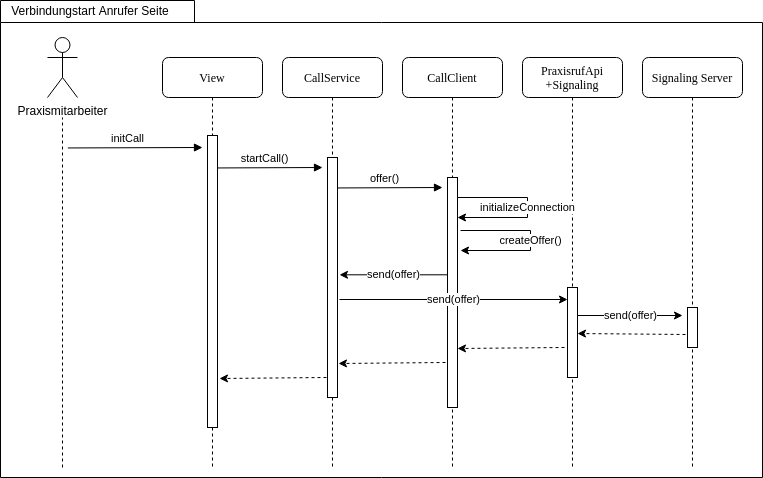
\includegraphics[width=\textwidth]{/home/joshua/FHNW/dev/IP6/IP6_Bachelorarbeit_Bericht_Cloudbasiertes_Praxisrufsystem/src/graphics/diagramms/Sequence_MobileClient_Caller_Signaling.drawio}
        \caption{Sequenzdiagramm - Verbindungsaufbau im Mobile Client}
    \end{minipage}
\end{figure}

Das versendete Signal wird über das Signaling Modul des Cloud Service an den Empfänger übermittelt.
Dieser empfängt das Signal über den SingalingClient.
Der SignalingClient gibt das Signal über onSignalReceived an den CallService weiter.
Der CallService aktiviert die Ansicht für aktive Anrufe und leitet das Signal an den CallClient weiter.
Der CallClient initialisiert die lokalen Verbindungsinformationen und erstellt eine Signal zur Bestätigung.
Dieses Signal wird wiederun über den CallService zum SignalingClient weiter zum Cloud Service versendet.
Auf Starterseite, kann diese Bestätigung weiterverarbeitet werden.

\subsubsection{Verpasste Anrufe}

Anrufe über die Gegensprechanlage können nur empfangen werden, solange die Praxisruf App im Vordergrund läuft und beim Signalingserver registriert ist.
Ist dies nicht der Fall, kann der Signalingserver keine Signale an den jeweiligen Empfänger zustellen.
Wenn der Singalingserver ein Signal für einen Empfänger erhält, der nicht verbunden ist wird versucht, diese über eine Benachrichtigung zu informieren.
Benachrichtigungen für verpasste Anrufe, werden gleich wie alle anderen Benachrichtigungen empfangen und in der Inbox angezeigt.
Für das Versenden der Benachrichtigung für verpasste Anrufe wird das bestehende Notification Modul des Cloudservice verwendet.
Dieses wird um einen Endpunkt erweitert, der es erlaubt Benachrichtigungen gezielt an einen einzelnen Client zu versenden.
Der neue Enpunkt nimmt zwei Parameter entgegen:
Die technische Identifikation des Empfängers und die technische Identifikation des relevanten Benachrichtigungstyps.
Der relevante Benachrichtigungstyp muss durch den Praxisadministrator im Admin UI erfasst werden.
Die technische Identifikation dieses Benachrichtigungstyps muss anschliessend in den Umgebungsvariablen des Signalingservices hinterlegt werden.\footnote{Vgl. Installationsanleitung}
Wenn der Empfänger nicht für Benachrichtigungen registriert ist, kann er nicht über den verpassten Anruf informiert werden.
Dasselbe gilt, wenn die Benachrichtigung aus technischen Gründen nicht zugestellt werden kann.
Im Rahmen dieses Projektes wird kein Mechanismus implementiert, um diese fehlgeschlagene Zustellung automatisch zu wiederholen.

\subsubsection{Deaktivierte Anrufe}

Praxismitarbeitende können das Empfangen von Anrufen lokal deaktivieren.
Wenn der Empfang von Anrufen deaktiviert ist, werden Offer Signale nicht mit einer Answer sondern mit einem Declined Signal beantwortet.
Empfängt ein Client ein Declined Signal, erstellt er lokal einen Eintrag in der Inbox und zeigt eine Push Benachrichtigung an um den Benutzer darauf hinzuweisen.

\subsubsection{Verbindungsende}

Praxismitarbeitende können Sprachverbindungen durch einen Button beenden.
Durch antippen des Auflagen-Buttons wird die bestehende Peer to Peer Verbindung zum Gesprächspartner getrennt.
Anschliessend wird ein Signal vom Typ End an die Gesprächspartner gesendet.
Durch Empfang des End-Signals, weiss der Gesprächspartner, dass die Verbindung durch das Gegenüber getrennt wurde und kann die Verbindung seinerseits entfernen.


\clearpage
